\documentclass[a4paper,11pt]{article}
\usepackage[T1]{fontenc}
\usepackage[utf8]{inputenc}
\usepackage{lmodern}
\usepackage{graphicx}
\usepackage[top=1in, bottom=1in, left=0.75in, right=1in]{geometry}

\usepackage{hyperref}
\hypersetup{
    colorlinks,
    citecolor=black,
    filecolor=black,
    linkcolor=black,
    urlcolor=black
}

\setlength{\parindent}{0cm}

\title{CS 435 Use Cases}

\author{
Taylor Flatt \\
at \\
Southern Illinois University of Carbondale
}

\begin{document}

\maketitle
\tableofcontents

%%%%%%%%%%%%%%%%%%%
% Start Section 1 %
%%%%%%%%%%%%%%%%%%%
\section{Use Case 1}
\subsection{Description}
This use case describes how a Flowchart User would register for an account to access the website.

\subsection{Actors}
\begin{enumerate}
\item Flowchart User
\item Flowchart System
\end{enumerate}

\subsection{Pre-Conditions}
\begin{itemize}
\item The User has an active internet connection which allows them to access the website.
\item The User must have an email address capable of receiving email.
\item The User must not already be logged into an account.
\end{itemize}

\subsection{Basic Flow of Events}
\begin{enumerate}
\item The use case begins when the user accesses the Registration webpage.
\item The User will enter an email account that they have access to and are able to receive email from.
\item The User enters a valid password.
\item The User confirms their password from step 3.
\item The user will be registered with the System provided they are validated and automatically logged into their account.
\end{enumerate}

\subsection{Alternative Flows}
\subsubsection{Already Registered}
If in step 4 in the basic flow, the System determines that the User is attempting to use an email that is already registered with our system, then
\begin{enumerate}
\item The User will be redirected to the login page.
\item A message will appear at the top of the page in red letters reading, "The account [Account Name] is already registered, please login to access the website".
\item The Use Case ends.
\end{enumerate}

\subsubsection{Invalid Email}
If in step 2 in the basic flow, the System determines that the email is in an incorrect format, then
\begin{enumerate}
\item The System will display a red box around the email field.
\item A popup bubble will appear next to the field indicating that the email is in the incorrect format and must be changed prior to continuing.
\item The use case continues at step 2.
\end{enumerate}

\subsubsection{Invalid Password}
If the user attempts to register with a password that does not fulfill the minimum password criteria, then
\begin{enumerate}
\item The System will display a red box around the password field.
\item A popup bubble will appear next to the field indicating that the password does not meet all of the password criteria and must be changed prior to continuing.
\item The use case continues at step 3.
\end{enumerate}

\subsubsection{Database Connection Lost}
If the System is attempting to validate the User's registration details and cannot access the database, then
\begin{enumerate}
\item The System will retry the database 3 times at 5 second intervals.
\item If the System cannot regain connectivity, then the User will be redirected to the Registration page indicating the error.
\item The use case ends in failure.
\end{enumerate}

\subsection{Post-Conditions}
\subsubsection{Successful Completion}
The user was able to register successfully and is now able to access the Flowchart website.

\subsubsection{Failure Condition}
The user is directed to the proper resource allowing them to rectify the issue.

\subsection{Special Requirements}
[SpReq:WC-1] The Flowchart System shall only allow one email address to be associated with a single user. Multiple registrations with the same email are not allowed.

\subsection{Diagram}
See \hyperref[fig:use-case-1]{Figure 1} below.

\texttt{\begin{figure}[hbtp]
\label{fig:use-case-1}
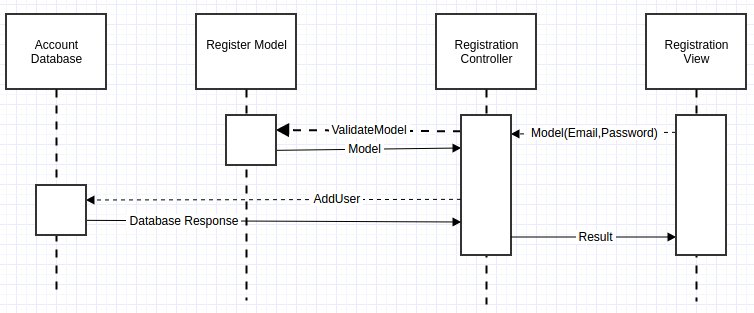
\includegraphics[scale=0.85]{use-case-1a.png}
\caption{Use Case 1 UML Diagram}
\end{figure}}

%%%%%%%%%%%%%%%%%%%
% Start Section 2 %
%%%%%%%%%%%%%%%%%%%
\section{Use Case 2}
\subsection{Description}
This use case describes how a User will login to the Flowchart Creator with their account.

\subsection{Actors}
\begin{enumerate}
\item Flowchart User
\item Flowchart System
\end{enumerate}

\subsection{Pre-Conditions}
\begin{itemize}
\item The User has an active internet connection which allows them to access the website.
\item The User must already be registered on the Flowchart website.
\item The User must not already be logged into an account.
\end{itemize}

\subsection{Basic Flow of Events}
\begin{enumerate}
\item The use case begins when the user accesses the Login webpage.
\item The User will enter an email account that they used to register.
\item The User enters their password.
\item The User will be logged in provided the Flowchart System authenticates the (email,password) combination.
\item Once successful, the user will be redirected to the homepage.
\end{enumerate}

\subsection{Alternative Flows}
\subsubsection{Already Logged In}
If in step 1 in the basic flow, the System determines that the User is already logged into an account, then
\begin{enumerate}
\item The User will be redirected to a landing page indicating that they are already logged in and that if they would like to login to another account, they must logout first. Links to the previous page as well as the homepage and a logout link will be provided as well.
\item The Use Case ends.
\end{enumerate}

\subsubsection{Incorrect Email}
If in step 4 in the basic flow, the System determines that the User has entered an email not contained within the database, then
\begin{enumerate}
\item The User will remain on the Login page.
\item A red box will appear around the email field.
\item A popup bubble will appear next to the field indicating "The email you have entered is incorrect. Please try again."
\item The use case continues at step 2.
\end{enumerate}

\subsubsection{Incorrect Password}
If in step 4 in the basic flow, the System determines that the User has entered an incorrect password, then
\begin{enumerate}
\item The User will remain on the Login page.
\item A red box will appear around the password field.
\item A popup bubble will appear next to the field indicating "The password you have entered is incorrect. Please try again."
\item The use case continues at step 3.
\end{enumerate}

\subsubsection{Database Connection Lost}
If the System is attempting to validate the User's Login details and cannot access the database, then
\begin{enumerate}
\item The System will retry the database 3 times at 5 second intervals.
\item If the System cannot regain connectivity, then the User will be redirected to the Login page indicating the error.
\item The use case ends in failure.
\end{enumerate}

\subsubsection{Invalid Login Attempts Exceeded}
If the System fails to validate the user more than 5 times within 10 minutes, then
\begin{enumerate}
\item The user will be locked out of their account for 10 minutes.
\item The use case ends in failure.
\end{enumerate}

\subsection{Post-Conditions}
\subsubsection{Successful Completion}
The user was able to login successfully and is now able to access the Flowchart website. The logs have been updated reflecting the successful login.

\subsubsection{Failure Condition}
The user is directed to the proper resource allowing them to rectify the issue. The logs have been updated reflecting the unsuccessful login.

\subsection{Special Requirements}
[SpReq:WC-1] The Flowchart System shall maintain a log of all authentication attempts which will include IP, email, timestamp, and authentication outcome.

\subsection{Diagram}
\texttt{\begin{figure}[hbtp]
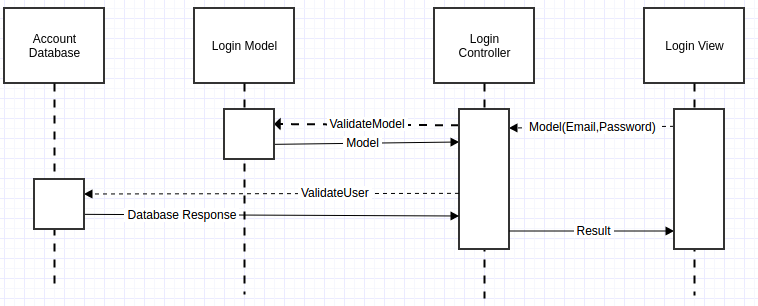
\includegraphics[scale=0.85]{use-case-2a.png}
\caption{Use Case 2 UML Diagram}
\end{figure}}

\end{document}
